\chapter{Architecture\\
\small{\textit{-- Nikhil Kumar G, Raj Palival}}
\index{Chapter!Architecture}
\index{Architecture}
\label{Chapter::Architecture}}

\section{Description\label{Section::ArchitectureIntro}}
OpenCV (Open Source Computer Vision Library \cite{OCV}) is an open-source library that includes several hundreds of computer vision algorithms. It has a modular structure architecture, which means that the package includes several modules with shared or static libraries. 

\section{Modules \label{subSection::ModulesList}}
There are two types of modules available:
\begin{enumerate}
     \item Main Modules: These modules are the core components of the OpenCV library that provide essential computer vision functionalities.
     \item Extra modules: These are additional modules that offer extended features and algorithms not included in the main modules.
 \end{enumerate}
Below is a list of all the modules available in each category:

\subsection{Main Modules\label{subSection::MainModules}}
\begin{enumerate}
     \item core. Core functionality: a compact module defining basic data structures, including the dense multi-dimensional array Mat and basic functions used by all other modules. \index{Core functionality}
     \item imgproc. Image Processing: an image processing module that includes linear and non-linear image filtering, geometrical image transformations (resize, affine and perspective warping, generic table-based remapping), color space conversion, histograms, and so on. \index{Image Processing}
     \item imgcodecs. Image file reading and writing: This module in OpenCV provides functions for reading and writing image files in various formats \index{imgcodecs}
     \item videoio. Video I/O: This module in OpenCV provides functions for reading and writing video files and accessing video streams from cameras or other devices. \index{videoio}
     \item highgui. High-level GUI: This module in OpenCV provides high-level functions for creating graphical user interfaces (GUI) to display and interact with images, videos, and other visual data. \index{High-level GUI}
     \item video. Video Analysis: This module in OpenCV involves performing various operations on video frames, such as object detection, tracking, motion analysis, and frame manipulation. \index{object detection}
     \item calib3d. Camera Calibration and 3D Reconstruction: This module in OpenCV provides functions for camera calibration and 3D reconstruction. \index{Camera Calibration}
     \item features2d. 2D Features Framework: This module in OpenCV provides a framework for detecting and describing 2D image features. These features can be used for tasks such as image matching, object recognition, and image stitching. \index{2D Features Framework}
     \item objdetect. Object Detection: This module in OpenCV provides functions and pre-trained models for object detection. It allows you to detect and localize objects within images or video frames.\index{objdetect}
     \item dnn. Deep Neural Network module: This module in OpenCV provides a flexible and efficient framework for working with deep neural networks (DNNs). It allows you to load pre-trained models, perform inference on images or videos, and fine-tune models. \index{Deep Neural Network}
     \item ml. Machine Learning: This module in OpenCV provides a set of machine learning algorithms and tools for various tasks, including classification, regression, clustering, and dimensionality reduction.\index{Machine Learning}
     \item flann. Clustering and Search in Multi-Dimensional Spaces: This module in OpenCV provides efficient algorithms for clustering and searching in multi-dimensional spaces. FLANN stands for Fast Library for Approximate Nearest Neighbors. \index{Clustering}
     \item photo. Computational Photography: This module refers to the use of computational techniques and algorithms to enhance or modify digital photographs.\index{Computational Photography} 
     \item stitching. Images stitching: Image stitching is the process of combining multiple overlapping images to create a larger, seamless panorama. \index{Images stitching}
     \item gapi. Graph API: This module is a computational graph-based framework provided by OpenCV that allows for efficient parallel execution of image processing and computer vision algorithms. \index{Graph API}
 \end{enumerate}
 \subsection{Extra Modules\label{subSection::ExtraModules}}
\begin{enumerate}
     \item alphamat. Alpha Matting \index{Alpha Matting}
     \item aruco. Aruco markers, module functionality was moved to objdetect module \index{Aruco markers}
     \item barcode. Barcode detecting and decoding methods \index{Barcode detecting}
     \item bgsegm. Improved Background-Foreground Segmentation Methods \index{Segmentation}
     \item bioinspired. Biologically inspired vision models and derivated tools \index{bioinspired}
     \item ccalib. Custom Calibration Pattern for 3D reconstruction
     \item cudaarithm. Operations on Matrices
     \item cudabgsegm. Background Segmentation
     \item cudacodec. Video Encoding/Decoding
     \item cudafeatures2d. Feature Detection and Description
     \item cudafilters. Image Filtering
     \item cudaimgproc. Image Processing
     \item cudalegacy. Legacy support
     \item cudaobjdetect. Object Detection
     \item cudaoptflow. Optical Flow
     \item cudastereo. Stereo Correspondence
     \item cudawarping. Image Warping
     \item cudev. Device layer
     \item cvv. GUI for Interactive Visual Debugging of Computer Vision Programs
     \item datasets. Framework for working with different datasets
     \item dnn objdetect. DNN used for object detection
     \item dnn superres. DNN used for super resolution
     \item dpm. Deformable Part-based Models
     \item face. Face Analysis
     \item freetype. Drawing UTF-8 strings with freetype/harfbuzz
     \item fuzzy. Image processing based on fuzzy mathematics
     \item hdf. Hierarchical Data Format I/O routines
     \item hfs. Hierarchical Feature Selection for Efficient Image Segmentation
     \item img hash. The module brings implementations of different image hashing algorithms.
     \item intensity transform. The module brings implementations of intensity transformation algorithms to adjust image contrast.
     \item julia. Julia bindings for OpenCV
     \item line descriptor. Binary descriptors for lines extracted from an image
     \item mcc. Macbeth Chart module
     \item optflow. Optical Flow Algorithms
     \item ovis. OGRE 3D Visualiser
     \item phase unwrapping. Phase Unwrapping API
     \item plot. Plot function for Mat data
     \item quality. Image Quality Analysis (IQA) API
     \item rapid. silhouette based 3D object tracking
     \item reg. Image Registration
     \item rgbd. RGB-Depth Processing
     \item saliency. Saliency API
     \item sfm. Structure From Motion
     \item shape. Shape Distance and Matching
     \item stereo. Stereo Correspondance Algorithms
     \item structured light. Structured Light API
     \item superres. Super Resolution
     \item surface matching. Surface Matching
     \item text. Scene Text Detection and Recognition
     \item tracking. Tracking API
     \item videostab. Video Stabilization
     \item viz. 3D Visualizer
     \item wechat qrcode. WeChat QR code detector for detecting and parsing QR code.
     \item xfeatures2d. Extra 2D Features Framework
     \item ximgproc. Extended Image Processing
     \item xobjdetect. Extended object detection
     \item xphoto. Additional photo processing algorithms
\end{enumerate}

\section{Grouping Modules\label{Section::GroupingModules}}
The modules don't have a clear order or hierarchy. Core, python, and java are commonly used modules, but there isn't a definite separation between them. Often, a module that uses the core module also depends on another module, which makes the structure very complex.\\\\
However, we can group all the modules in three categories:
\begin{enumerate}
     \item Main Functionality
     \item Extended Functionality
     \item High Level GUI
\end{enumerate}

\section{15 Most Important Modules\label{Section::HighLevelView}}
Below is a figure of the 15 most important modules in the three categories discussed above:
\begin{figure}[H]
     \centering
     \scalebox{0.8}{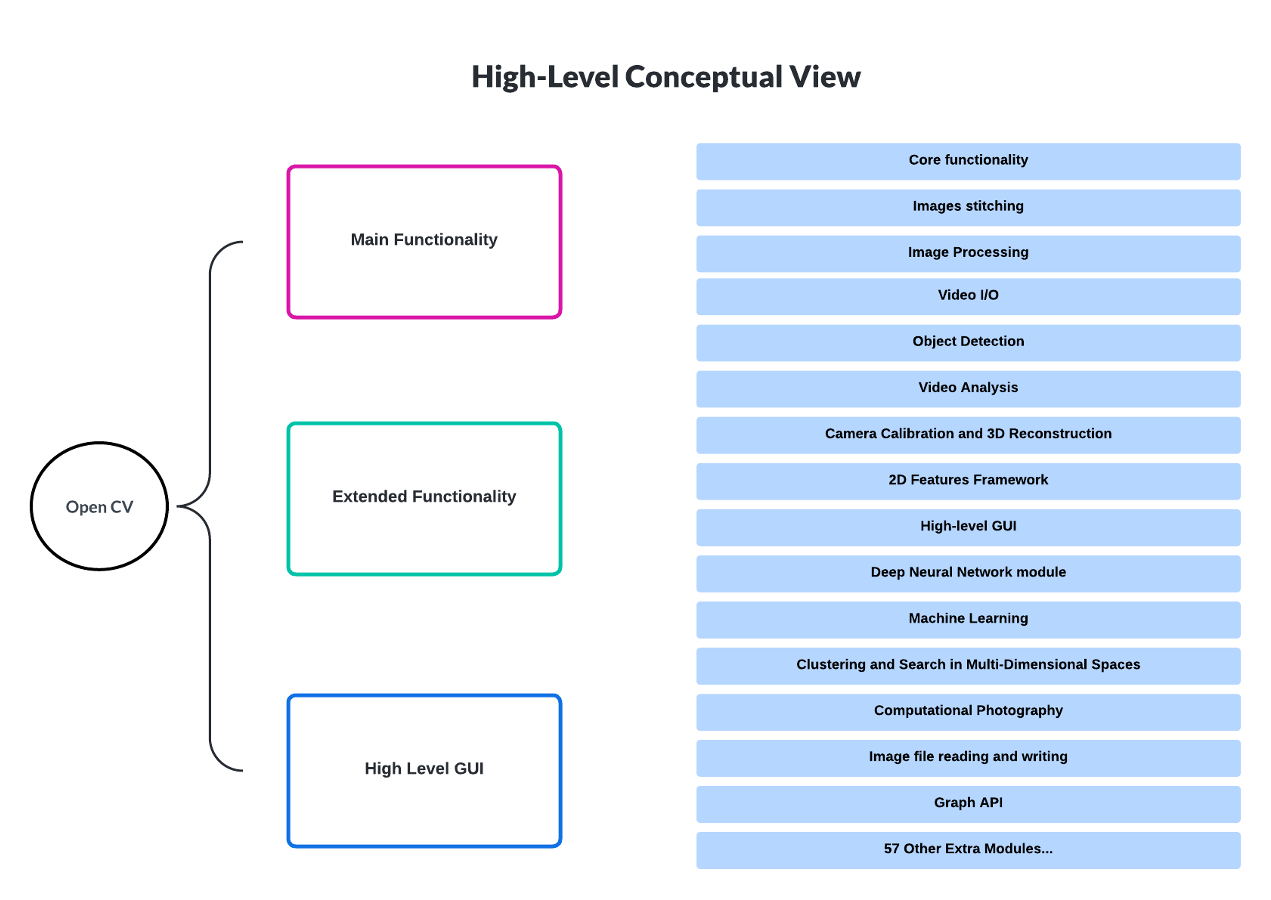
\includegraphics{Figures/Conceptualview.png}}
     \caption{\label{Figure::HighLevelView} High Level Conceptual View}
\end{figure}
\pagebreak

\section{4+1 View of Architecture\label{Section::4+1view}}
The 4+1 architectural view model provides multiple perspectives on the architecture of a system \cite{UNB}. Such as:
\begin{enumerate}
         \item Implementation View
         \item Use Case View
         \item Logical View
         \item Process View
         \item Deployment View
\end{enumerate}
We will use an example of one module to explain the rest of the OpenCV modules in OpenCV’s architecture. More on this later.
\subsection{Implementation View\label{subSection::ImplementationView}} \index{Implementation View}
The implementation view is an architectural view that  provides a detailed perspective on how the system is implemented and how the implementation artifacts are organized and interact with each other.\\\\
     In our case we will consider the following:
     \begin{itemize}
         \item Perspective: Developers, Proj. mngs.
         \item Stage: Design
         \item Focus: Subsystem decomposition
         \item Concerns: Software management
         \item Artefacts: Modules structure, Package diagram
     \end{itemize}
\subsubsection{Implementation View Artefacts\label{subsubSection::ImplementationView}} \index{Artefacts}
The modules structure below shows how all the modules in OpenCV interact with each other. It is clear that the modules in OpenCV are interconnected in a very complex way. \\\\

Modules Structure: Diagram taken from source \cite{OGB} 

\begin{figure}[H]
     \centering
     \scalebox{0.15}{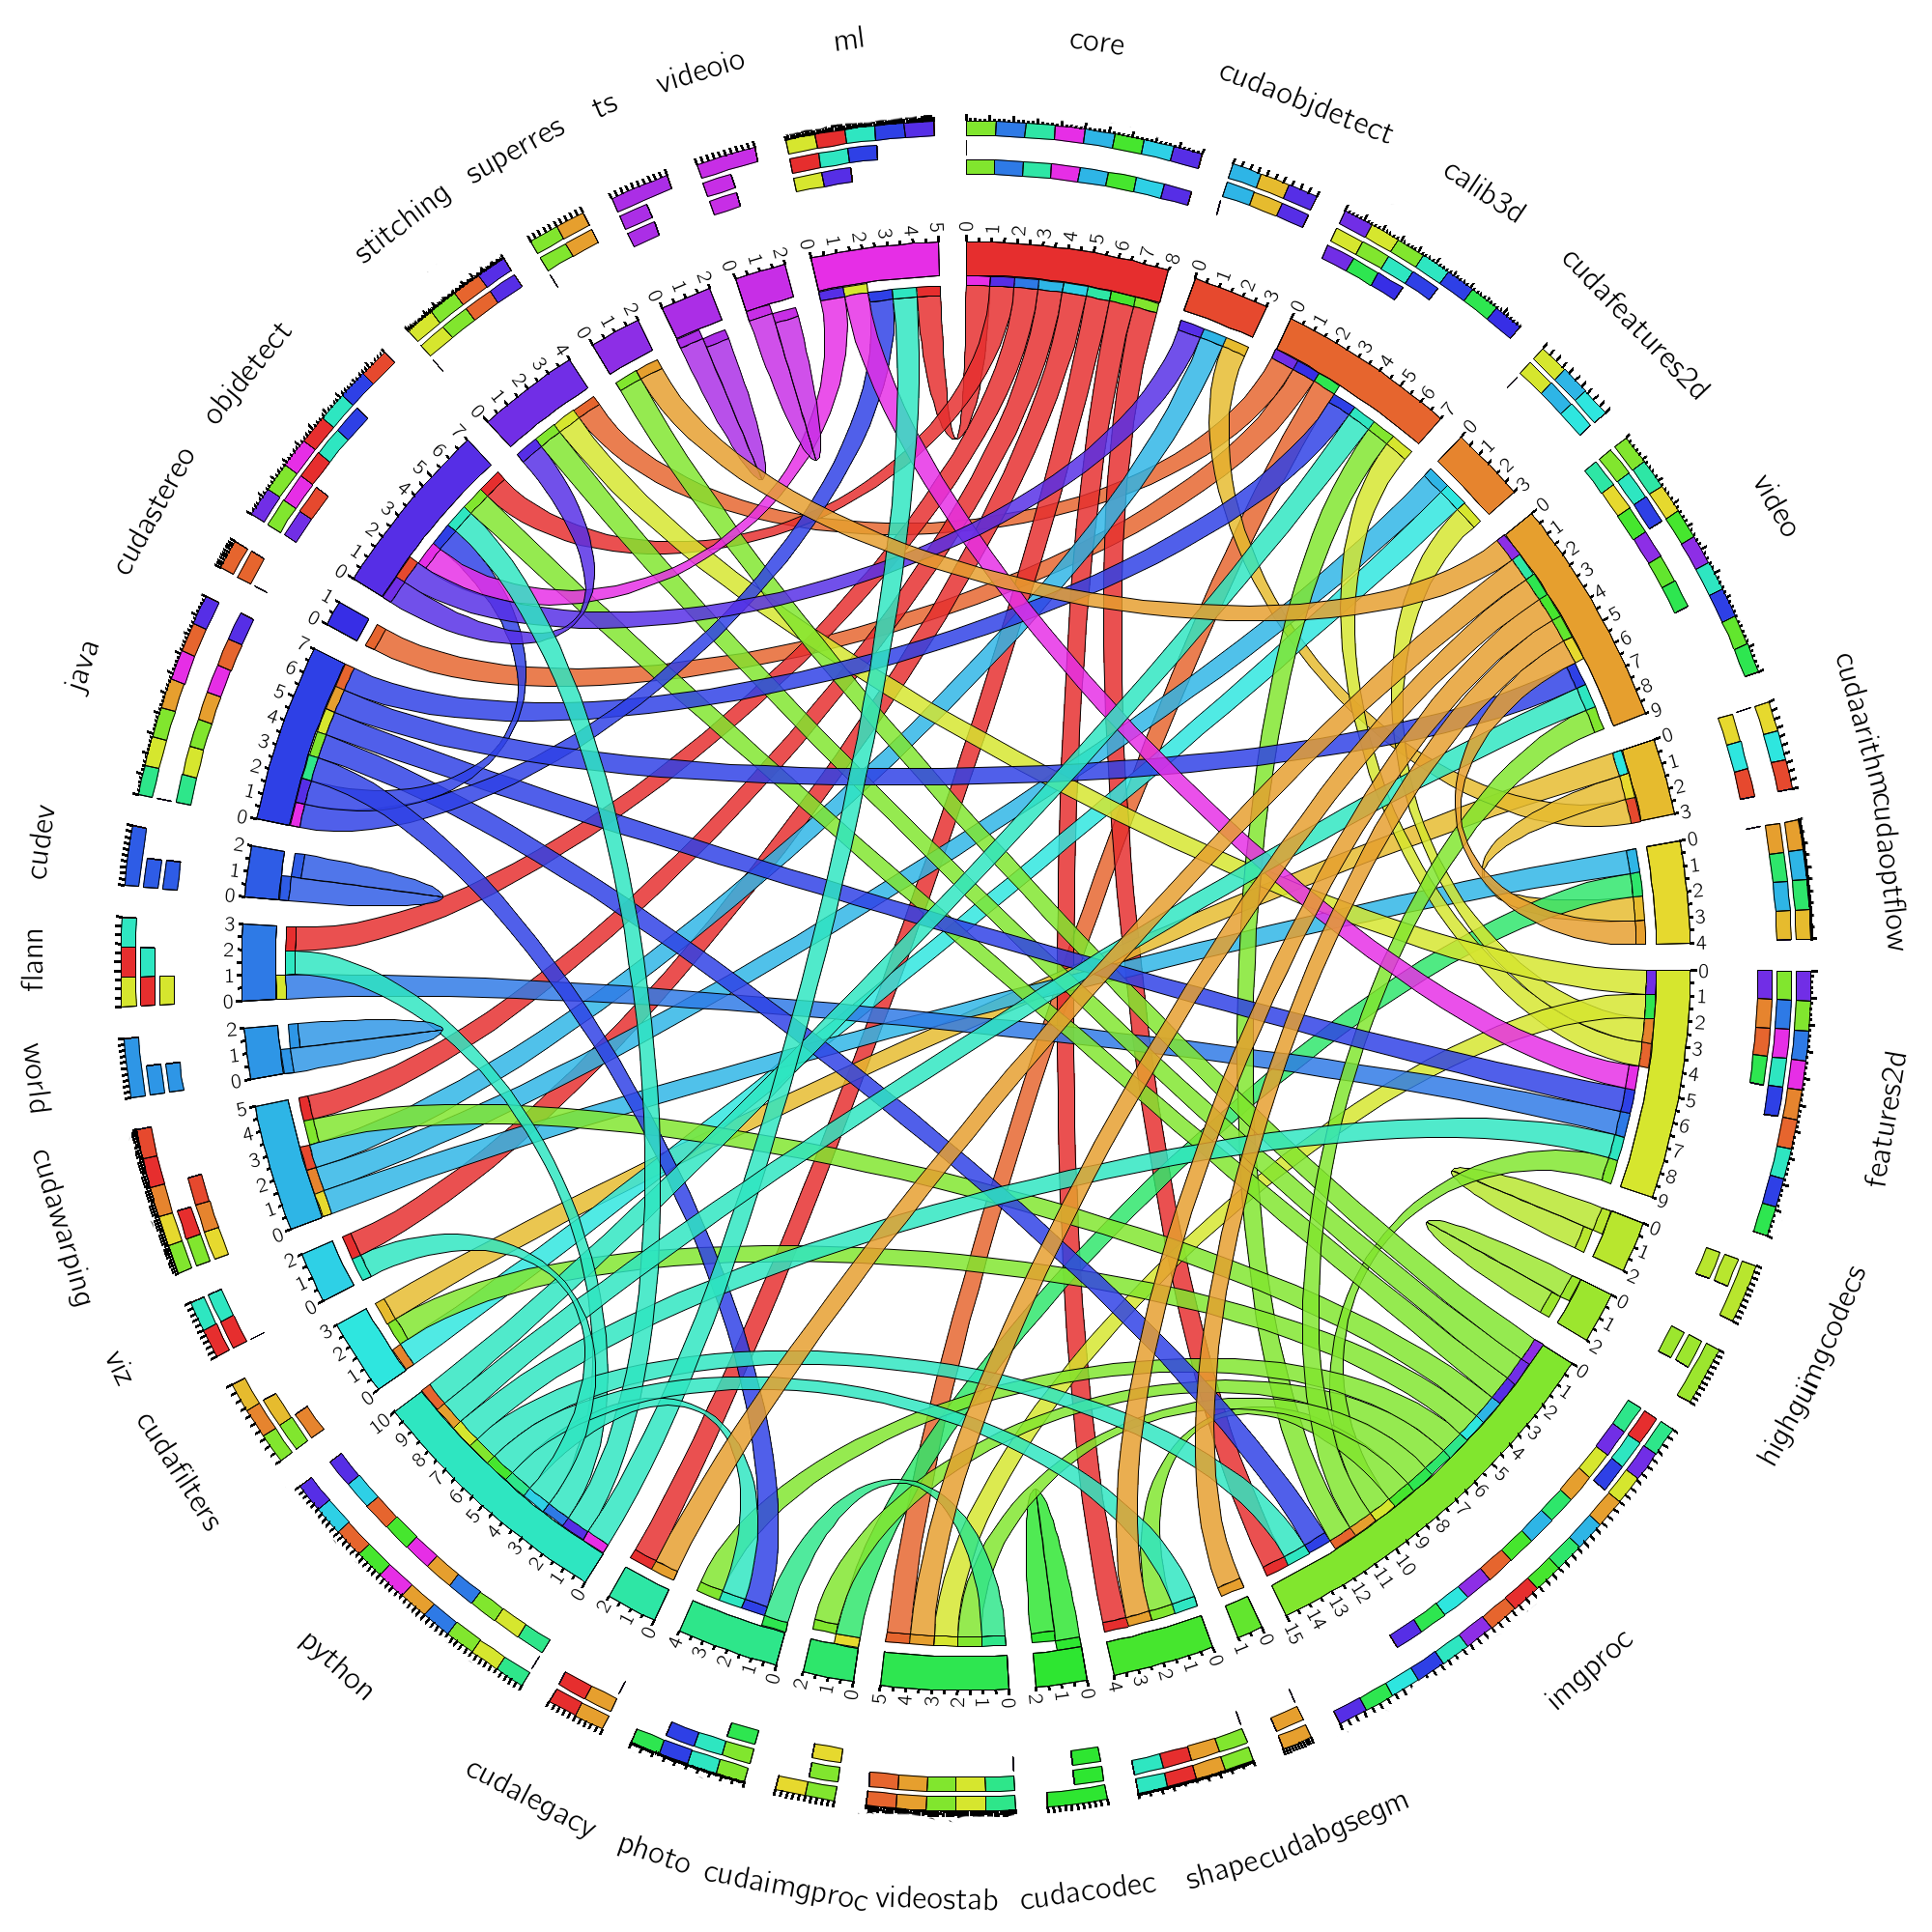
\includegraphics{Figures/ModulesStructure.png}}
     \caption{\label{Figure::ModulesStructure} Modules Interconnection Structure}
\end{figure}
Because of its complex nature, we will zoom into the architecture a little bit and understand one such important module of OpenCV among the 15 most important modules through all the 4+1 views' from here on:
\begin{itemize}
         \item Image Stitching Module (stitching.): Famously used to create panorama images \cite{6896208}. \index{panorama} 
\end{itemize}
The idea is to understand this one module which in-turn sort of explains the rest of the OpenCV modules in OpenCV's architecture. \\\\
Below is a Package Diagram of Image Stitching Module:\\\\
The diagram includes 3 levels:
\begin{enumerate}
         \item 1st Level: It is the OpenCV package that contains all modules.
         \item 2nd Level: It shows how the Image Stitching module is Interacting with other modules in OpenCV package.
         \item 3rd Level: Shows the functions present in Image Stitching module and the other two modules.
\end{enumerate}

\begin{figure}[H]
     \centering
     \scalebox{0.5}{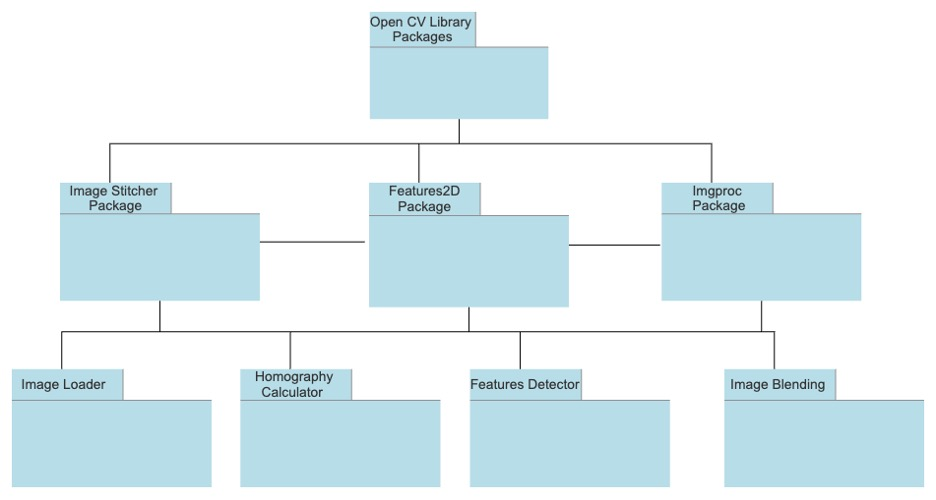
\includegraphics{Figures/PackageDiagram.jpg}}
     \caption{\label{Figure::ImageStitcherPackageDiagram
} Image Stitcher Package Diagram}
\end{figure}

\subsubsection{Functions\label{subsubSection::Functions}}
\begin{enumerate}
         \item Image Loader: It is used to load and prepare the images in Image Stitching package for stitching process.
         \item Homography Calculator: It is used to calculate a homography matrix between two sets of corresponding points in an image. \index{Homography}
         \item Features Detector: It is used to identify and extract distinctive features or points of interest from an image.
         \item Image Blending: It is the process of combining two or more images to create a single composite image that preserves the important information from each input image. \index{Image Blending}
\end{enumerate}
\pagebreak

\subsection{Use Case View\label{subSection::UserCaseView}} \index{User Case View}
The use case view is an architectural view that focuses on describing the system's functionality from the perspective of its users or external actors.\\\\
     In our case we will consider the following:
     \begin{itemize}
         \item Perspective: End users
         \item Stage: Putting it alltogether
         \item Concerns: Understandability, usability
         \item Focus: Feature decomposition
         \item Artefact: Use-case diagram
     \end{itemize}

\subsubsection{Use Case Diagram\label{subsubSection::UseCaseDiag}}
\begin{figure}[H]
     \centering
     \scalebox{0.68}{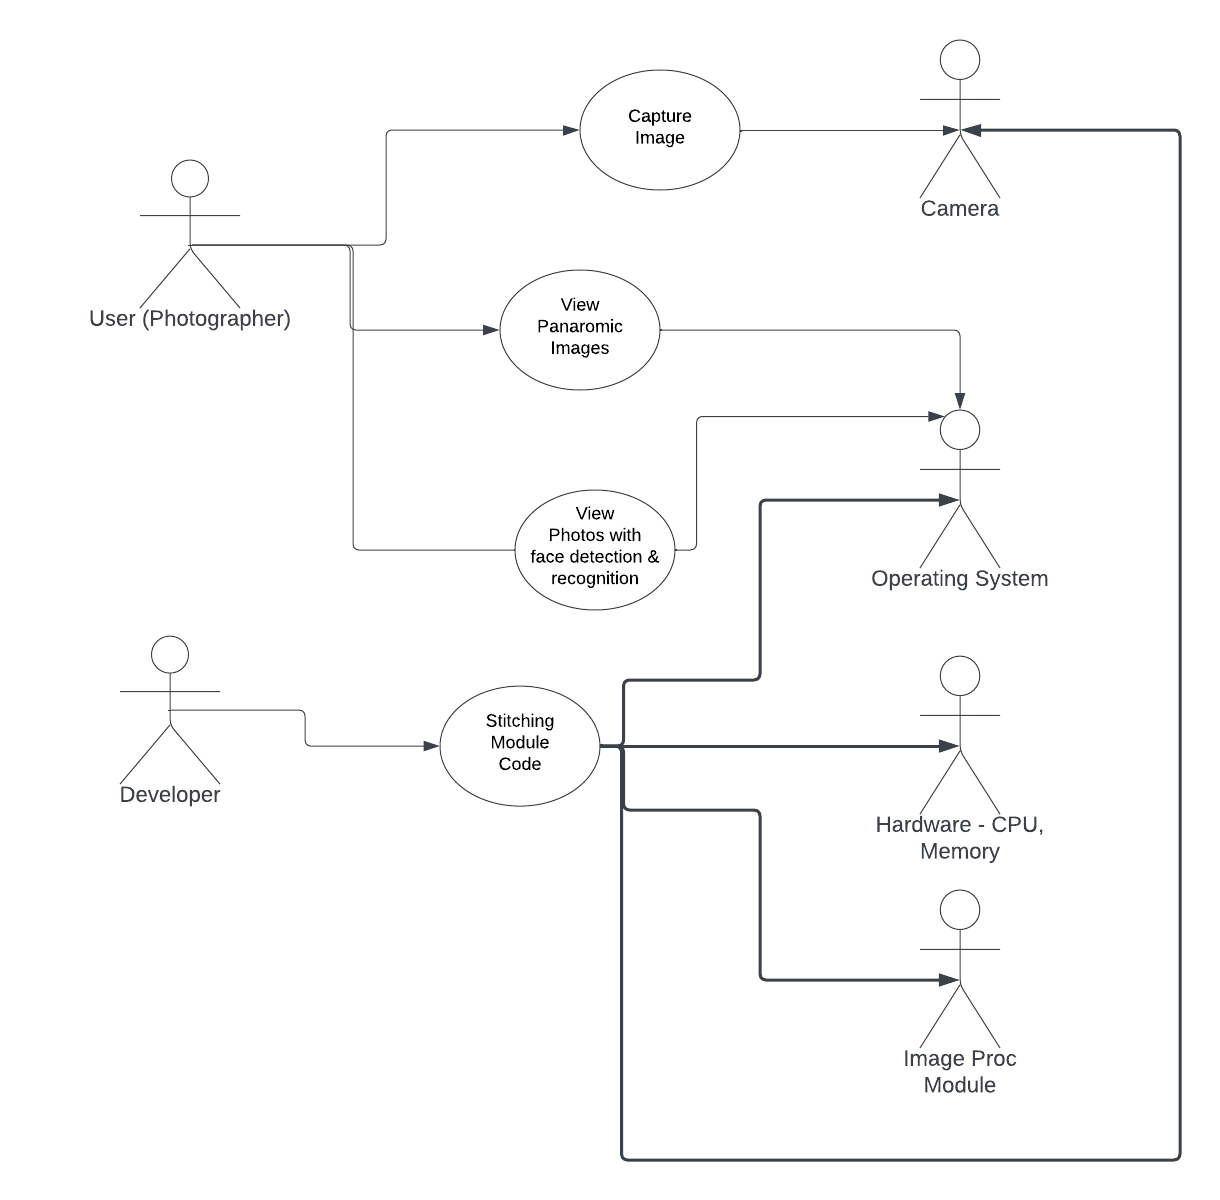
\includegraphics{Figures/Use Case Diagram of ImageStitchingModule.png}}
     \caption{\label{Figure::UseCaseDiagram
} Use Case Diagram for Image Stiching Module \cite{lucidchart}}
\end{figure}

We have the following in our diagram:
\begin{enumerate}
         \item Actors: Two actors \index{Actors}
         \begin{enumerate}
         \item User: Photographer has 3 use cases:- \index{Photographer}
             \begin{enumerate}
             \item To capture images
             \item View panaromic images
             \item View photos with face detection and recognition.
             \end{enumerate}
         \item Developer has 1 use case:- \index{Developer}
             \begin{enumerate}
             \item Develop stitching module code
             \end{enumerate}
\end{enumerate}
         \item Use Cases: Four use cases 
         \begin{enumerate}
             \item To capture images
             \item View panaromic images
             \item View photos with face detection and recognition.
             \item Develop stitching module code
         \end{enumerate}

         \item External Actors: Four external actors
         \begin{enumerate}
             \item Camera: Facilitates in capturing images \index{Camera}
             \item Operating System: Used by both User and developer for their use cases \index{Operating System}
             \item Hardware Components: CPU, Memory \index{CPU} \index{Memory}
             \item Image Proc Module: Provides a wide range of functions and algorithms for manipulating and enhancing images.
         \end{enumerate}
         
\end{enumerate}


\pagebreak

\subsection{Logical View\label{subSection::LogicalView}} \index{Logical View}
The logical view is an architectural view that focuses on representing the high-level structure and organization of the system's functionality and behavior. It provides an abstraction of the system's functionality and its relationships, without delving into implementation details. \\\\
     In our case we will consider the following:
     \begin{itemize}
         \item Perspective: Analysts, Designers Stage: Requirement analysis \index{Analysts}
         \item Focus: Object oriented decomposition
         \item Concerns: Functionality
         \item Artefacts: Class diagram \cite{UMLdiagram}
     \end{itemize}

\begin{figure}[H]
     \centering
     \scalebox{0.6}{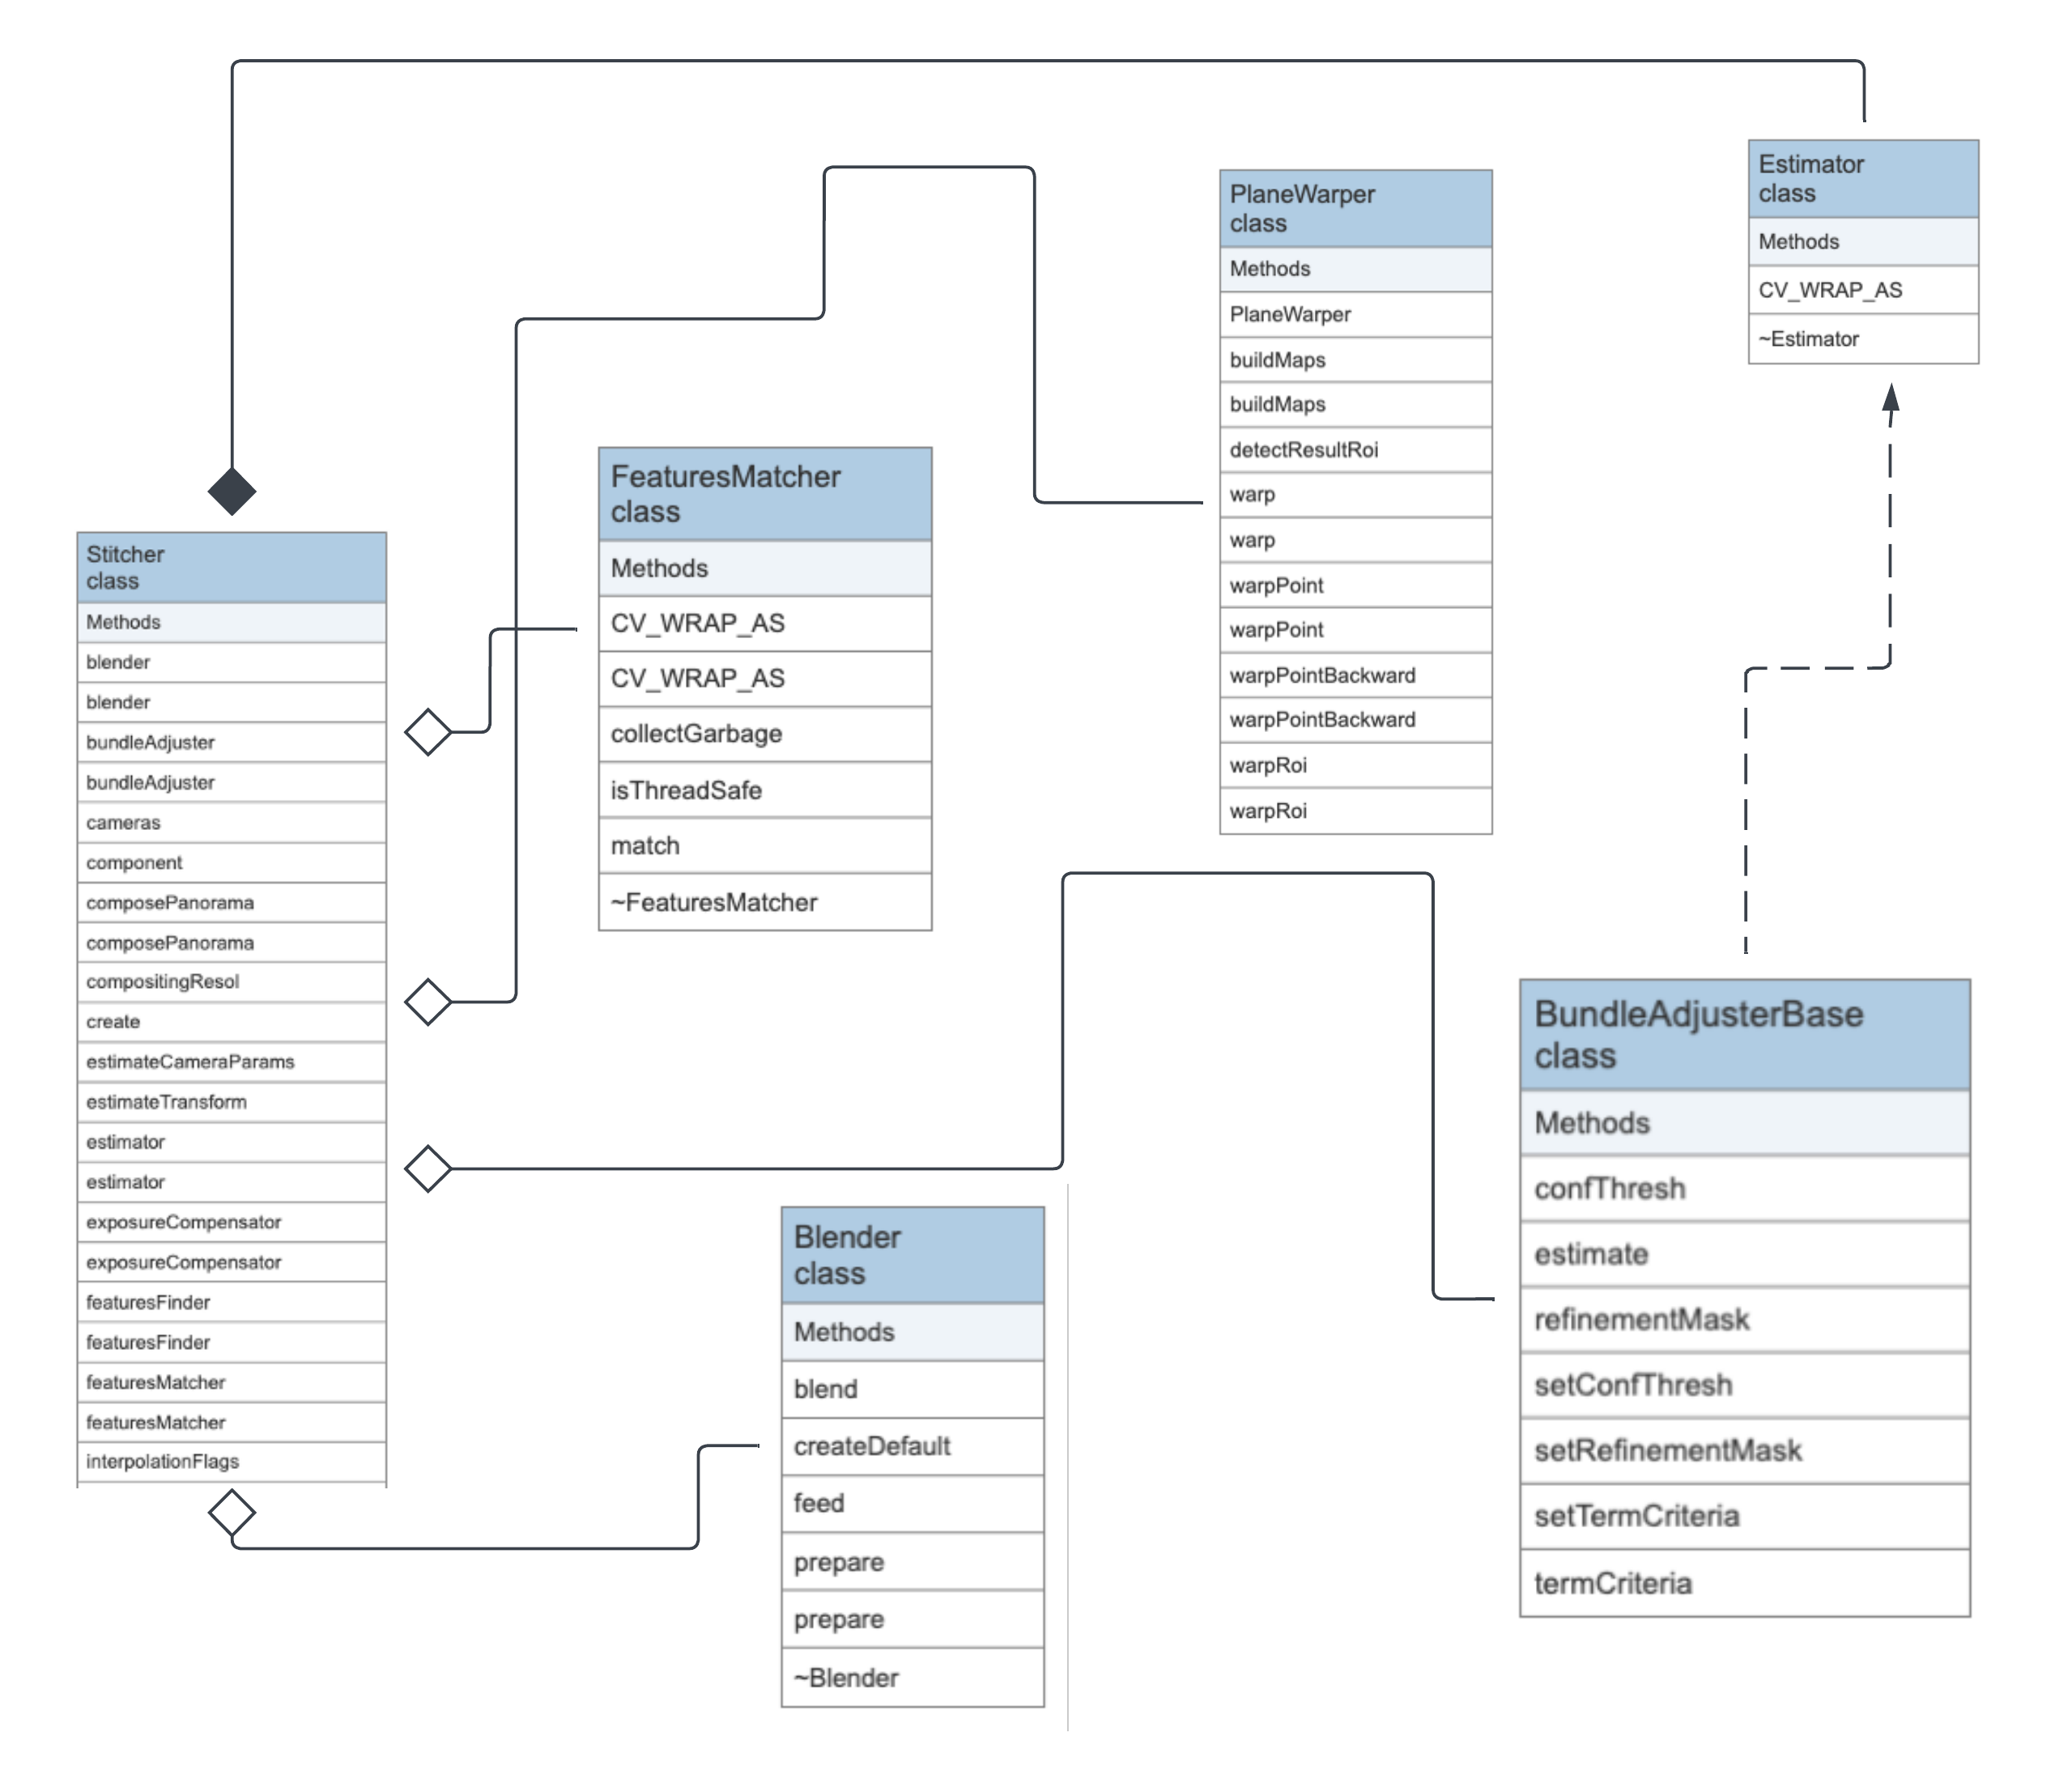
\includegraphics{Figures/ClassDiagram.png}}
     \caption{\label{Figure::BriefOverview} Class Diagram of Image Stitching Module \cite{smartdraw}}
\end{figure}
The logical view of OpenCV's Image Stitching module describes the system's functionality and the relationships between its components. The module consists of several classes, including the Stitcher class, Features Matcher class, Plane Warper class, Blender class, BundleAdjusterBaseClass, and Estimator class. Here is a brief description of each class and how they depend on each other:
\begin{enumerate}
    \item Stitcher class: The Stitcher class is the main class in the Image Stitching module. It provides the functionality to stitch multiple images together to create a panoramic image. The Stitcher class uses other classes in the module to perform various tasks, such as feature detection, feature matching, and image blending.
    \item Features Matcher class: The Features Matcher class is responsible for detecting and matching features in the input images. It uses various algorithms to detect and match features, such as the SIFT algorithm and the SURF algorithm.
    \item Plane Warper class: The Plane Warper class is responsible for warping the input images to a common plane. It uses various algorithms to perform the warping, such as the Homography algorithm and the Affine algorithm.
    \item Blender class: The Blender class is responsible for blending the warped images together to create a seamless panoramic image. It uses various algorithms to perform the blending, such as the Multi-band blending algorithm and the Feather blending algorithm.
    \item BundleAdjusterBaseClass: The BundleAdjusterBaseClass is responsible for adjusting the parameters of the stitching process to improve the quality of the output image. It uses various algorithms to adjust the parameters, such as the Levenberg-Marquardt algorithm and the Gauss-Newton algorithm.
    \item Estimator class: The Estimator class is responsible for estimating the camera parameters of the input images. It uses various algorithms to estimate the parameters, such as the RANSAC algorithm and the Least Squares algorithm.\\
\end{enumerate}
These classes depend on each other in a hierarchical manner. The Stitcher class is the main class that uses the other classes to perform various tasks. The Features Matcher class and the Estimator class are used by the Stitcher class to detect and match features and estimate camera parameters, respectively. The Plane Warper class is used by the Stitcher class to warp the input images to a common plane. The Blender class is used by the Stitcher class to blend the warped images together to create a seamless panoramic image. Finally, the BundleAdjusterBaseClass is used by the Stitcher class to adjust the parameters of the stitching process to improve the quality of the output image. Overall, these classes work together to provide the functionality of the Image Stitching module in OpenCV.
\pagebreak


\subsection{Process View\label{subSection::ProcessView}}
The process view is an architectural view that focuses on illustrating the runtime behavior and concurrency aspects of a system. It provides a perspective on how the system's functionality is executed and how different components or processes interact and collaborate during runtime.\\\\
     In our case we will consider the following:
     \begin{itemize}
         \item Perspective: System Integrators \index{System Integrators}
         \item Stage: Design
         \item Focus: Process decomposition
         \item Concerns: Performance, scalability, throughput \index{throughput}
         \item Artefacts: Sequence diagram \index{Sequence diagram}
     \end{itemize}
     
\subsubsection{Sequence Diagram\label{subsubSection::SequenceDiag}}
\begin{figure}[H]
     \centering
     \scalebox{0.38}{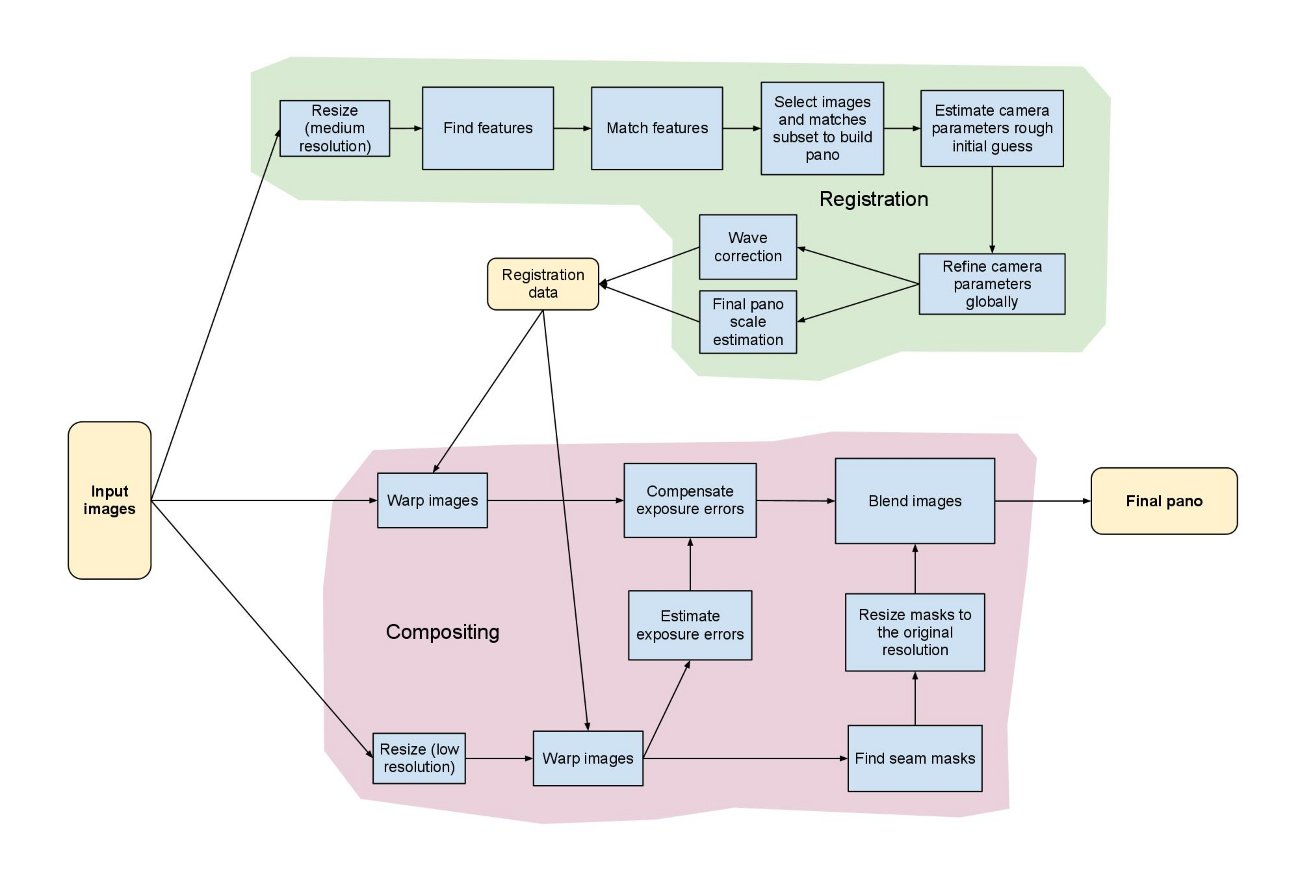
\includegraphics{Figures/StitchingPipeline.jpg}}
     \caption{\label{Figure::StitchingPipeline} Sequence Diagram of Image Stitching Module} \index{Stitching Pipeline}
\end{figure}
The process view of OpenCV's Image Stitching module describes the system's behavior and how it responds to external events. The module performs several operations to stitch multiple images together to create a panoramic image. Here is a brief description of each operation and the steps involved:
\begin{enumerate}
    \item Step 1 - Input Images:\\ The first operation is to input the images that need to be stitched together. These images are typically captured using a camera or downloaded from a source.

    \item Step 2 - Registration:\\ The second operation is registration, which involves several steps:
    \begin{itemize}
        \item Resize (medium resolution): The input images are resized to a medium resolution to reduce the computational complexity of the feature detection and matching algorithms.
        \item Find features: The feature detection algorithm is used to detect features in the input images, such as corners, edges, and blobs.
        \item Match features: The feature matching algorithm is used to match the features between the input images.
        \item Select images and matches subset to build panorama: The input images and their corresponding feature matches are selected to build the panorama.
        \item Estimate camera parameters rough initial guess: The camera parameters of the input images are estimated using a rough initial guess.
        \item Refine camera parameters globally: The camera parameters are refined globally using a bundle adjustment algorithm.
        \item Wave correction: The wave correction algorithm is used to correct the distortion caused by the camera lens.
        \item Final panorama scale estimation: The final scale of the panorama is estimated based on the camera parameters and the input images.
    \end{itemize}

    \item Step 3 - Registration data :\\ The registration data, including the camera parameters and the warped images, are passed to the compositing operation.

    \item Step 4 - Compositing:\\ The final operation is compositing, which involves several steps:
    \begin{itemize}
        \item Warp images: The warped images are transformed to a common coordinate system using the estimated camera parameters.
        \item Estimate exposure errors: The exposure errors in the input images are estimated using an exposure estimation algorithm.
        \item Compensate exposure errors: The exposure errors in the input images are compensated using an exposure compensation algorithm.
        \item Resize (low resolution): The final panoramic image is resized to a low resolution for display or storage purposes.
        \item Warp images: The warped images are transformed again to the original resolution.
        \item Find seam masks: The seam masks are found using a seam finding algorithm.
        \item Resize masks to original resolution: The seam masks are resized to the original resolution.
        \item Blend images: The blended image is created by blending the warped images together using a blending algorithm.
    \end{itemize}
    \item Step 5 - Final panorama:\\ The final panoramic image is created by combining the blended image and the seam masks.
\end{enumerate}
Overall, the process view of OpenCV's Image Stitching module describes the system's behavior and how it responds to external events, such as input images and user requests. The module performs several operations, including registration and compositing, to stitch multiple images together to create a beautiful panoramic image.
\pagebreak

\subsection{Deployment View\label{subSection::DeploymentView}}
The deployment view is an architectural view that focuses on illustrating how the software components of a system are deployed and distributed across hardware resources. It provides a representation of the physical infrastructure and deployment topology of the system.\\\\ \index{Deployment View}
     In our case we will consider the following:
     \begin{itemize}
         \item Perspective: System Engineers
         \item Stage: Design
         \item Focus: Map software to hardware
         \item Concerns: System topology, delivery, installation, communication
         \item Artefacts: Deployment diagram
     \end{itemize}

\subsubsection{Deployment Diagram\label{subsubSection::DeploymentDiag}}
\begin{figure}[H]
     \centering
     \scalebox{0.9}{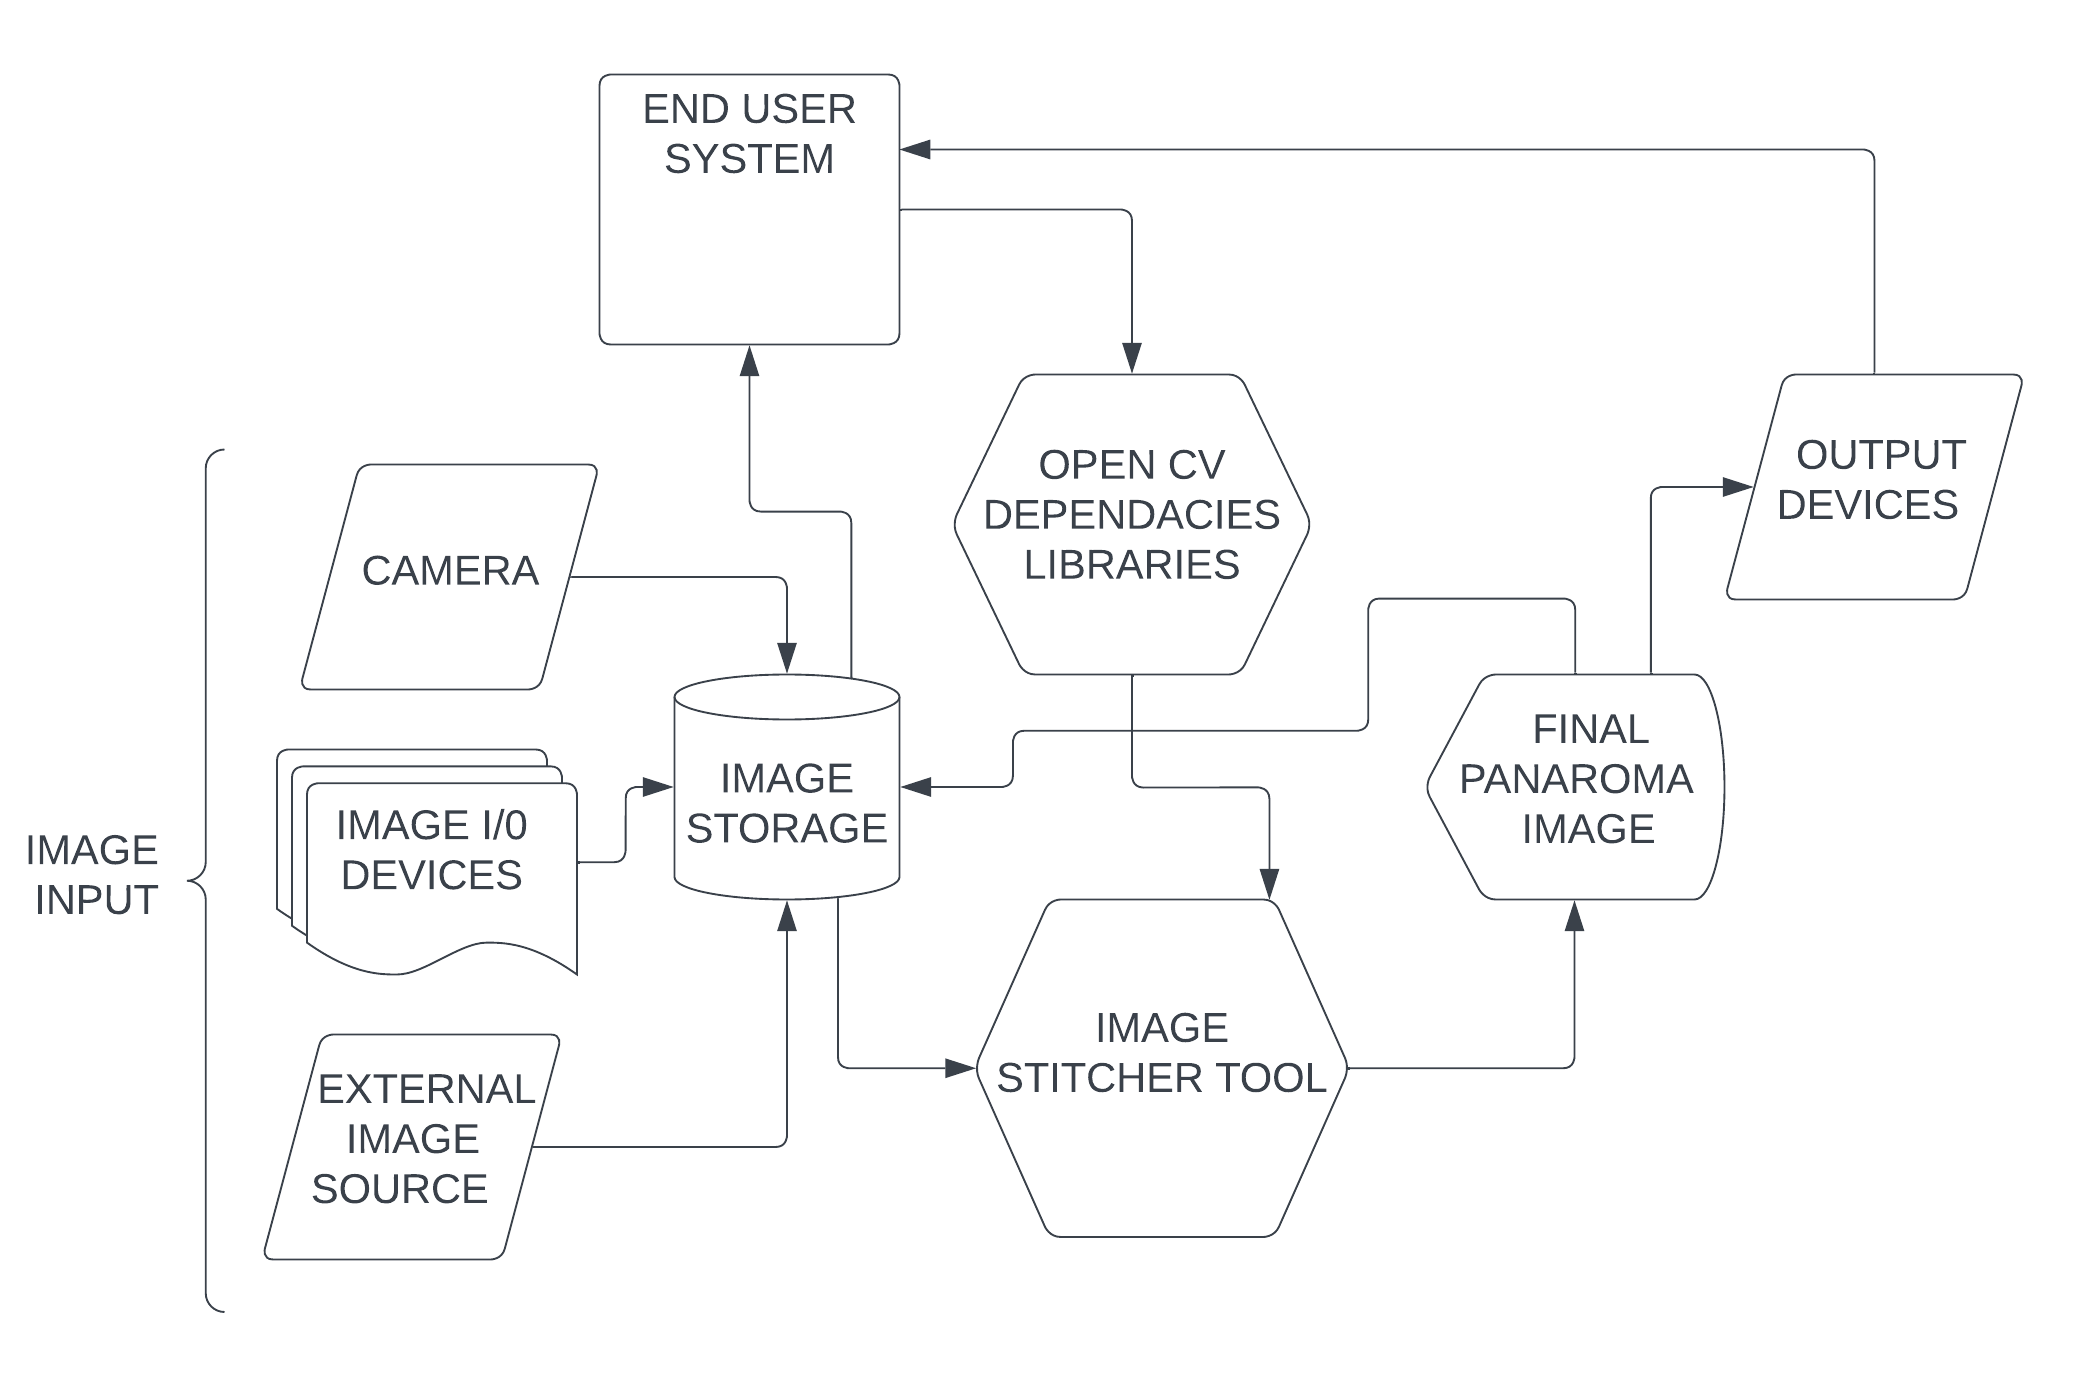
\includegraphics{Figures/DeploymentDiagram.png}}
     \caption{\label{Figure::DeploymentDiagram} Deployment Diagram of Image Stitching Module}
\end{figure}
The deployment view of OpenCV's image stitching module involves several components that work together to produce a final panorama output image: 
\begin{enumerate}
    \item Image input: The images that need to be stitched together.
    \begin{itemize}
        \item Camera: This is the device that captures the images that will be stitched together. 
        \item Image input/output devices: These are devices that can be used to input or output images, such as USB drives or SD cards. 
        \item External image source: This component refers to any external source of images that can be used as input for the stitching process.
    \end{itemize}
    \item Image storage database: This component is responsible for storing the images that will be used for stitching. It can be a local or remote database.

    \item OpenCV libraries / dependencies: This component includes all the necessary libraries and dependencies required for the image stitching module to function properly.

    \item Image Stitching module of OpenCV: This is the core component of the deployment view. It is responsible for stitching the input images together to produce a final panorama output image.

    \item Final panorama output image: This is the output of the image stitching module. It is the final image that is produced after the input images have been stitched together.

    \item Output devices: These are devices that can be used to output the final panorama image, such as a monitor or a printer.

    \item End-user system: This component refers to the system that the end-user will be using to access the image stitching module. It can be a desktop computer, a laptop, or a mobile device.
\end{enumerate}
Overall, the deployment view of OpenCV's image stitching module involves several components that work together to produce a final panorama output image. The input images can come from various sources, and the final output can be displayed on different output devices. The image stitching module is the core component that stitches the input images together, and the end-user system is the system that the end-user will be using to access the module.
\subsubsection{OpenCV Installation Dependencies\label{subsubSection::opencvInstallation}}
To install OpenCV on a system, there are several dependencies that need to be installed first. The specific dependencies required may vary depending on the operating system and the version of OpenCV being installed. Here is a general list of dependencies that are commonly required:
\begin{enumerate}
    \item CMake: This is a cross-platform build system that is used to build OpenCV from source.
    \item Git: This is a version control system that is used to download the OpenCV source code.
    \item GCC: This is a compiler that is used to compile the OpenCV source code.
    \item Python: OpenCV has a Python interface, so Python needs to be installed on the system.
    \item NumPy: This is a Python library that is used for numerical computing. It is required for the Python interface of OpenCV.
    \item libjpeg: This is a library for reading and writing JPEG files. It is required for the imgcodecs module of OpenCV.
    \item libpng: This is a library for reading and writing PNG files. It is required for the imgcodecs module of OpenCV.
    \item libtiff: This is a library for reading and writing TIFF files. It is required for the imgcodecs module of OpenCV.
    \item libjasper: This is a library for reading and writing JPEG-2000 files. It is required for the imgcodecs module of OpenCV.
    \item libwebp: This is a library for reading and writing WebP files. It is required for the imgcodecs module of OpenCV.
    \item OpenEXR: This is a library for reading and writing high dynamic range (HDR) images. It is required for the imgcodecs module of OpenCV.
    \item TBB: This is the Intel Threading Building Blocks library, which is used for parallel processing. It is required for the performance optimization of OpenCV.
    \item Eigen: This is a C++ template library for linear algebra. It is used for the computation of homography matrices in the image stitching process.
    \item CUDA: This is a parallel computing platform and programming model developed by NVIDIA. It is used for GPU acceleration in the image stitching process.
    \item OpenCL: This is an open standard for parallel programming of heterogeneous systems. It is used for GPU acceleration in the image stitching process.
\end{enumerate}
\pagebreak

\section{Summary of 4+1 View:\label{Section::Overview}}
Each view provides a distinct perspective on the OpenCV architecture, allowing stakeholders to understand and analyze the system from different angles. This 4+1 view model helps in capturing the functional, development, process, physical, and use case aspects of the OpenCV backend architecture.\\\\ \index{Backend}
Here is a diagram to showcase a brief overview of what we covered:

\begin{figure}[H]
     \centering
     \scalebox{0.23}{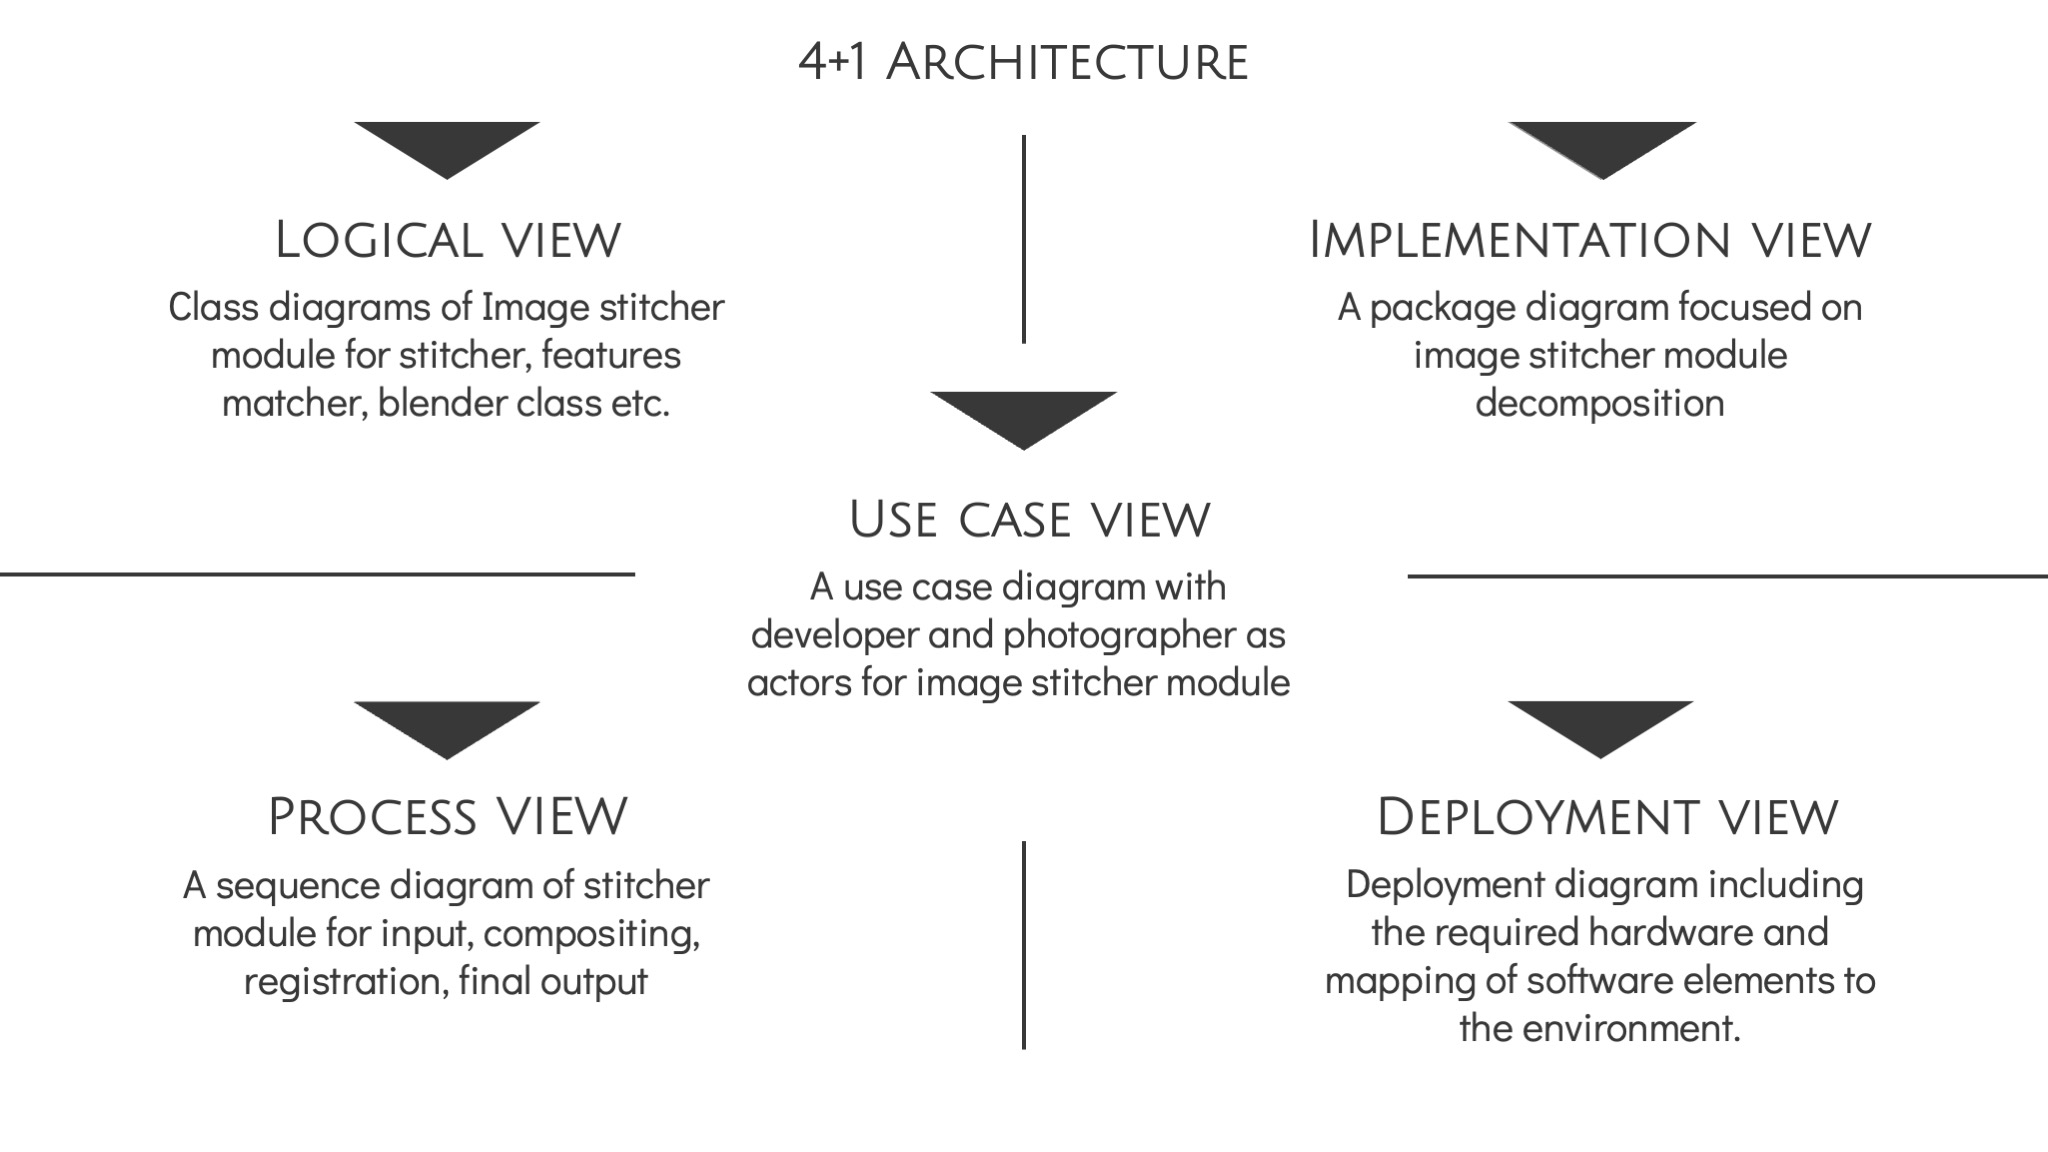
\includegraphics{Figures/BriefOverview.jpg}}
     \caption{\label{Figure::BriefOverview} 4+1 Overview}
\end{figure}
\par{The purpose of using the 4+1 view model for OpenCV's Image Stitching module is to provide a comprehensive understanding of the system's architecture from multiple perspectives. This approach helps to ensure that the system is designed and implemented in a way that meets the needs and requirements of its stakeholders, while also addressing potential risks and quality issues. \index{4+1 view}\\
\\
The Logical View provides a high-level overview of the system's functionality and the relationships between its components. This view focuses on the system's data and functionality, and how they are organized and structured. It helps stakeholders to understand the system's overall purpose and how it achieves its goals.\\
\\
The Process View describes the system's behavior and how it responds to external events. This view focuses on the system's processes and how they interact with each other and with external systems. It helps stakeholders to understand how the system works and how it responds to different inputs and events.\\
\\
The Implementation View describes the system's development environment and how it is organized. This view focuses on the system's development tools, processes, and methodologies. It helps stakeholders to understand how the system is developed and maintained, and how changes are made to the system over time.\\
\\
The Deployment View describes the system's physical architecture and how it is deployed. This view focuses on the system's hardware and software components, and how they are connected and configured. It helps stakeholders to understand how the system is deployed and how it interacts with other systems and devices.\\
\\
The Use Case View describes the system's functionality from the perspective of its users. This view focuses on the system's use cases and how they are implemented in the system. It helps stakeholders to understand how the system is used and how it meets the needs and requirements of its users.
\vspace{20pt}\\
Overall, the 4+1 view model provides a comprehensive understanding of the OpenCV Image Stitching module's architecture from multiple perspectives, helping stakeholders to understand the system's functionality, behavior, development environment, physical architecture, and user requirements. This understanding is essential for ensuring that the system is designed and implemented in a way that meets the needs and requirements of its stakeholders, while also addressing potential risks and quality issues.
}





